\documentclass[a4paper]{article}

\usepackage[T2A]{fontenc}
\usepackage[russian, english]{babel}
\usepackage{multicol} %колонки
\usepackage{setspace} %межстрочный интервал
\usepackage{fancyhdr} %настройки верхнего и нижнего колонтитулов в документе.
\usepackage{scrextend}
\usepackage{float}
\usepackage{caption}
\usepackage{biblatex}
\usepackage{enumitem}
\usepackage{mathtools}
\usepackage[left=2.5cm,right=2.5cm,top=2.5cm,bottom=2.5cm]{geometry}
\usepackage{titlesec}


\pagestyle{fancy}
\makeatletter
\newcommand*{\rom}[1]{\expandafter\@slowromancap\romannumeral #1@}
\makeatother
\captionsetup{font=small}
\fancyhf{} % очищает все верхние и нижние колонтитулы.
\renewcommand{\headrulewidth}{0pt}
\fancyfoot[C]{\textbf{\thepage}}
\setcounter{page}{186}% настройка нумерации страниц 
\setlength{\columnsep}{0.4cm} % интервал между колонками
\titleformat{\section}{\normalsize\centering}{\thesection. }{0cm}{}[]

\begin{document}
\setlength\parindent{11pt}
\fontsize{10}{11}\selectfont


\begin{multicols}{2}
 \renewcommand{\labelenumi}{\theenumi)} % Римские цифры
 \begin{enumerate} [itemsep=-5pt, labelsep=5pt] % Настройка отступов
     \item Railway lines and stations: This subject area describes information about various railway lines,
including their geographical location, length, speed
limits, track types, and accessibility. It also includes information about stations, including their
location, capacity, and cargo and passenger handling capabilities.
\item Cargoes and containers: This subject area describes
various types of cargoes and containers, their characteristics (weight, volume, type of packaging), processing and storage requirements. It also includes information about special requirements for
certain types of goods, for example, goods requiring special transportation conditions (temperature
conditions, vibration protection, etc.).
\item Schedule and Train Timetable: This subject area
describes information about the train timetable,
including departure and arrival times, intermediate stops, travel speeds and possible overlaps on
the track. It also includes information about the
regularity and repeatability of the train schedule.
\item Resources: This subject area describes information about available resources such as locomotives, wagons, personnel, and technical equipment.
It includes the characteristics of resources (load
capacity, technical parameters), their availability
and maintenance schedule. 
\item Laws and Regulations: This subject area describes
the laws, rules and regulations governing railway
logistics. It includes safety rules, standards for the
transportation of certain goods, requirements for
staff working hours, rules for the priority of train
traffic and other regulatory information.
\item {Monitoring and Data collection: This subject area
describes the monitoring and data collection systems used to obtain information about the current
state of railway logistics. It includes data on train
movement, cargo status, information about delays
and other factors affecting planning and management.}
 \end{enumerate}
{\vspace{-0.2cm} \hspace{0.3cm}} Various problem solvers can be used to automate transportation planning and management. Here are some
typical problem solvers that can be applied in this field:

\renewcommand{\labelenumi}{\theenumi)} % Римские цифры
\begin{enumerate} [itemsep=-5pt, labelsep=5pt]
 
 \item The routing problem solver: This solver allows
you to optimize train routes, taking into account
various factors such as schedules, availability of
railway lines, cargo requirements and restrictions
on infrastructure and transportation conditions. It
helps to choose the best routes, minimizing the
time and cost of transportation.
\item Train timetable development solver: This solver
allows to optimize the train timetable, taking into
account the timetable, passenger and cargo requirements, infrastructure constraints and other factors.
It helps to allocate trains by time and resources, 
\item Loading planning problem solver: This solver helps
to optimize the loading of wagons, taking into
account the characteristics of goods and limitations
of wagons, such as load capacity, dimensions and
special requirements. It helps to maximize the
loading of wagons, minimizing empty runs and
improving the use of the wagon fleet.
\item The solver of the optimal resource planning problem: This solver allows you to optimize the allocation of resources such as locomotives, wagons,
personnel and technical equipment to ensure the efficient operation of the railway system. It takes into
account transportation requirements, traffic schedules and resource constraints, helping to achieve
optimal use of resources and reduce costs.
\item Demand Forecasting and Planning Solver: This
solver is used to predict the demand for rail
transportation, taking into account various external
factors such as economic conditions, seasonality,
trends and others. It helps to plan capacity and
resources to meet demand and prevent congestion
or lack of transportation capacity.
\item Monitoring and Management Problem Solver: This
solver is used for continuous monitoring and management of railway transportation. It analyzes data
on train movements, traffic status, delays and other
events, allowing you to make operational decisions
and respond to changes in real time.
\end{enumerate}
{\hspace{0.2cm}} These are just some examples of problem solvers that
can be used to automate the planning and management of
railway logistics. The specific set of solvers will depend
on the specific requirements and characteristics of the
railway logistics system, as well as on the goals and
constraints set.
{\hspace{0.2cm}} Using ontology for these problem solvers in the field
of railway logistics can bring several advantages: \par
\renewcommand{\labelenumi}{\theenumi)}
\begin{enumerate} [itemsep=-5pt, labelsep=5pt]
    \item Knowledge structuring: Ontology allows you to
structure knowledge about the main subject areas of railway logistics, such as infrastructure,
resources, cargo and schedules. This facilitates
the understanding and organization of information,
simplifies its accessibility and exchange between
different systems and participants.
    \item Data unification and standardization: An ontology
defines common semantics and standards for data
representation in railway logistics. This allows different systems and applications to use the same
terms and data formats, which ensures consistency
and compatibility of information. This is especially
important when integrating different systems and
exchanging data between them.
    \item Improvement of planning and optimization: Ontology provides a formalized domain model on the basis of which planning and optimization algorithms can be developed. The use of ontology makes it possible to take into account various limitations, requirements and dependencies between different aspects of railway logistics. This contributes to more efficient use of resources, route optimization and improved service quality.
    \item Decision Making Improvement: Ontology can be
used in decision support systems, providing a semantic model and context for data analysis and
recommendation generation. It allows systems to
identify dependencies and relationships between
various factors, to carry out forecasting and scenario analysis, which helps to make reasonable and
informed decisions.
    \item Ease of expansion and modification: Ontology
provides a flexible and extensible domain model
that can be easily modified and supplemented as
needed. This allows you to adapt the ontology to
new requirements, changing conditions and expand
its functionality. This flexibility makes it easier to
support different types of tasks and to develop the
system in the future.
\end{enumerate} 

In general, the use of ontology for data solvers in the field of railway logistics contributes to improving data
organization, information compatibility and consistency,
optimizing planning and management processes, as well
as making informed decisions based on data analysis.

The ontology for these problem solvers in the field of transportation process management should be flexible
and modular in order to take into account various factors
and adapt to changing conditions.
\setcounter{figure}{1}
\begin{figure}[H]
    \centering
    
\includegraphics[width=7.4cm]{1.PNG}
    \caption{Semantic neighborhood of knowlegebase RW}
    \label{fig:enter-label}
\end{figure}
Within the framework of this work, a top-level ontology is implemented describing the main objects of the
transportation process, examples of objects of which are
presented in Figures 2-4 in the form of an SCg code [10].
\begin{center}
  \rom{5.} Conclusion  
\end{center} \par
\fontsize{10}{10}\selectfont
Thus, within the framework of this work, the relevance
of developing an ontology for an intelligent transportation process management system has been determined.
\begin{figure}[H]
    \centering
    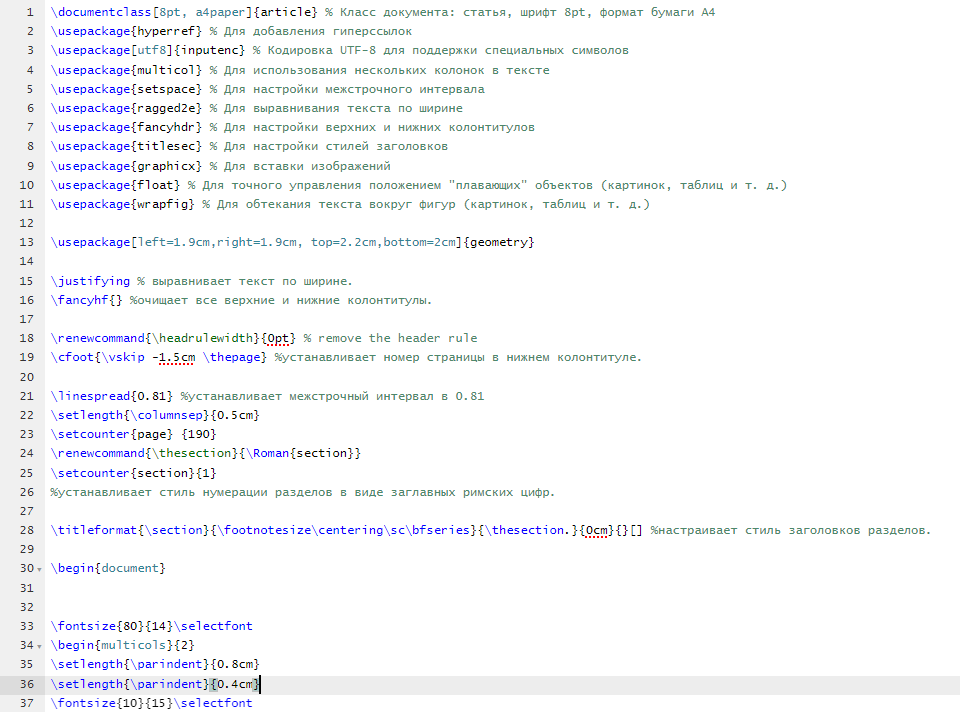
\includegraphics[width=7.4cm]{2.PNG}
    \caption{Semantic neighborhood of knowlegebase RW}
    \label{fig:enter-label}
\end{figure}
\begin{figure}[H]
    \centering
    \includegraphics[width=7.4cm]{3.PNG}
    \caption{Semantic neighborhood of static objects RW}
    \label{fig:enter-label}
\end{figure}
\fontsize{10}{10}\selectfont
The structure of the theory of ontology construction
is given. The existing ontologies of railway systems
are described. The problems of existing ontologies are
established. It is proposed to use a process-object approach in the formation of ontology. Examples of the
use of ontology are given. It is indicated that the OSTIS
technology is an effective tool for describing the process-
object ontology of the transportation process. The top-
level ontology for the Belarusian Railway has been
implemented.
\fontsize{8}{9}\selectfont
\begin{thebibliography}{10}
    \bibitem{bookl} A. A. Erofeev Intelectualnaya sistema upravlenia
perevozochnim processom [Intelligent control system
for the transportation pro- cess in railway transport].
The Ministry of Education of the Re- public. Belarus,
Belarusian state University of Transport. Gomel,
BSUT, 2022, P. 407
\bibitem{bookl} A. P. Badeckii, O. A. Medved Ontologicheskii podhod
k razrabotke edinoi basi znanii multimodalnih perevo-
zok [An ontological approach to the development of
a unified knowledge base for multimodal transporta-
tion]. Proceedings of the St. Petersburg University of
Railway Engineering, 2023, № 1, pp. 182–193
\bibitem{bookl} Ontology Description Capture IDEF5. https://www.idef.
com/idef5-ontology-description-capture-method/
(Accessed 10.03.2024)
\bibitem{bookl} T. Gruber Toward Principles for the Design of On-
tologies Used for Knowledge Sharing. Int. Journal
Human-Computer Studies, Vol. 43, pp. 907–928.
\bibitem{bookl} A. D. Obuhov Ontology neshtatnih situacii na sor-
tirovochnoi stancii po nepriemu poezda [Ontology of
emergency situations at the marshalling yard because
of unreception of trains]. Mate- rials of the IV Inter-
national Scientific and Practical Conference "Modern
concepts of scientific researchers", N. Novgorod, 2015,
pp. 281-284.
\bibitem{bookl} A. V. Borisov, A. V.Bosov, D. V.Zukov, A. V. Ivanov,
D. V. Sushko, Informationnie aspekti obespechenia
bezopasnosti na transporte: ontologiya predmetnoy
oblasti, modeli i varianti ispol- zovania [Information
aspects of transport safety: domain ontology, mod-
els and use cases], Systems and Means of Informat-
ics, Federal Research Center "Computer Science and
Control" of the Russian Academy of Sciences: 30:1
(2020), pp. 126–134
\bibitem{bookl} V. Golenkov and N. Guliakina, “Principles of building
mass semantic technology component design of intel-
ligent systems,” in Open semantic technologiesfor in-
telligent systems. Minsk, BSUIR, 2011, pp. 21–58 (in
Russian)
\bibitem{bookl} V. Golenkov and N. Gulyakina, “Semanticheskaya
tekhnologiya komponentnogo proektirovaniya sistem,
upravlyaemyh znaniyami [Semantic technology of
component design of knowledge-driven systems],” in
Open semantic technologiesfor intelligent systems,
Minsk, BSUIR, 2015, pp. 57–78, (in Russian)
\bibitem{bookl} V. V. Golenkov, “Ontology-based design of intelligent
systems,” in Open semantic technologies for intelli-
gent systems, ser. Iss. 1. Minsk : BSUIR, 2017, pp.
37–56.
\bibitem{bookl} V. V.Golenkov, Tehnologija kompleksnoj pod-
derzhki zhiznennogo cikla semanticheski sovmes-
timyh intellektual’nyh komp’juternyh sistem novogo
pokolenija [Technology of complex life cycle support
of semantically compatible intelligent computer sys-
tems of new generation ] – Minsk:Bestprint, 2023. P.
1063 (in Russian)
\end{thebibliography}
\columnbreak
\begin{center} 
\fontsize{14}{10}\selectfont {\textbf{ОСНОВЫ ОНТОЛОГИИ
ПЕРЕВОЗОЧНОГО ПРОЦЕССА НА
ЖЕЛЕЗНОДОРОЖНОМ ТРАНСПОРТЕ}}
\fontsize{12}{15}\selectfont
\par Ерофеев А. А., Ерофеев И. А.
\end{center}
\fontsize{10}{13}\selectfont
\hspace{0.2cm} Определена актуальность разработки онтологии для
интеллектуальной системы управления перевозочным
процессом. Приведена структура теории построения
онтологии. Описаны существующие онтологии желез-
нодорожных систем. Установлены проблемы суще-
ствующих онтологий. Предложено при формировании
онтологии использовать процессно-объектный под-
ход. Приведены примеры использования онтологии.
Указано, что эффективным инструментом описания
процессно-объектной онтологии перевозочного про-
цесса является технология OSTIS.
\begin{flushright}
    Received 13.03.2024
\end{flushright}
\end{multicols}
\end{document}
